\documentclass[dvips, lscape]{foils}
%\documentclass[dvips, french]{slides}
\textwidth 18.5cm
\textheight 25cm 
\topmargin -1cm 
\oddsidemargin  -1cm 
\evensidemargin  -1cm

% Maths
\usepackage{amsfonts, amsmath, amssymb, url}

\newcommand{\coefbin}[2]{\left( 
    \begin{array}{c} #1 \\ #2 \end{array} 
  \right)}
\renewcommand{\a}{\tt a}
\newcommand{\cc}{\tt c}
\newcommand{\g}{\tt g}
\renewcommand{\t}{\tt t}
\newcommand{\Dcal}{\mathcal{D}}
\newcommand{\Ecal}{\mathcal{E}}
\newcommand{\Ncal}{\mathcal{N}}
\newcommand{\Xbf}{{\bf X}}
\newcommand{\Bcal}{\mathcal{B}}
\newcommand{\Fcal}{\mathcal{F}}
\newcommand{\Lcal}{\mathcal{L}}
\newcommand{\Tcal}{\mathcal{T}}
\newcommand{\Ucal}{\mathcal{U}}
\newcommand{\mubf}{\mbox{\mathversion{bold}{$\mu$}}}
\newcommand{\Sigmabf}{\mbox{\mathversion{bold}{$\Sigma$}}}
\newcommand{\betabf}{\mbox{\mathversion{bold}{$\beta$}}}
\newcommand{\gammabf}{\mbox{\mathversion{bold}{$\gamma$}}}
\newcommand{\psibf}{\mbox{\mathversion{bold}{$\psi$}}}
\newcommand{\taubf}{\mbox{\mathversion{bold}{$\tau$}}}
\newcommand{\Rbb}{\mathbb{R}}
\newcommand{\Sbf}{{\bf S}}
% \newcommand{\bps}{\mbox{bps}}
\newcommand{\ubf}{{\bf u}}
\newcommand{\vbf}{{\bf v}}
\newcommand{\Esp}{{\mathbb E}}
% \newcommand{\Var}{{\mathbb V}}
\newcommand{\Ibb}{{\mathbb I}}
%\newcommand{\liste}{$\bullet \quad$}
\newcommand{\lFDR}{\ell FDR}

% Couleur et graphiques
\usepackage{color}
\usepackage{graphics}
\usepackage{epsfig} 
\usepackage{pstcol}

% Texte
\usepackage{lscape}
\usepackage{../../../../Latex/fancyheadings, rotating, enumerate}
%\usepackage[french]{babel}
\usepackage[latin1]{inputenc}
\definecolor{darkgreen}{cmyk}{0.5, 0, 0.5, 0.5}
\definecolor{orange}{cmyk}{0, 0.6, 0.8, 0}
\definecolor{jaune}{cmyk}{0, 0.5, 0.5, 0}
\newcommand{\textblue}[1]{\textcolor{blue}{#1}}
\newcommand{\textred}[1]{\textcolor{red}{#1}}
\newcommand{\textgreen}[1]{\textcolor{green}{ #1}}
\newcommand{\textlightgreen}[1]{\textcolor{green}{#1}}
\newcommand{\textdarkgreen}[1]{\textcolor{darkgreen}{#1}}
\newcommand{\textorange}[1]{\textcolor{orange}{#1}}
\newcommand{\textyellow}[1]{\textcolor{yellow}{#1}}
\newcommand{\refer}[2]{\textgreen{\sl #1}}
\newcommand{\emphase}[1]{\textblue{#1}}

% Sections
%\newcommand{\chapter}[1]{\centerline{\LARGE \textblue{#1}}}
% \newcommand{\section}[1]{\centerline{\Large \textblue{#1}}}
% \newcommand{\subsection}[1]{\noindent{\Large \textblue{#1}}}
% \newcommand{\subsubsection}[1]{\noindent{\large \textblue{#1}}}
% \newcommand{\paragraph}[1]{\noindent {\textblue{#1}}}
% Sectionsred
\newcommand{\chapter}[1]{
  \addtocounter{chapter}{1}
  \setcounter{section}{0}
  \setcounter{subsection}{0}
%   {\centerline{\LARGE \textblue{\arabic{chapter} - #1}}}
  {\centerline{\LARGE \textblue{#1}}}
  }
\newcommand{\section}[1]{
  \addtocounter{section}{1}
  \setcounter{subsection}{0}
%   {\centerline{\Large \textblue{\arabic{chapter}.\arabic{section} - #1}}}
  {\centerline{\Large \textblue{#1}}}
  }
\newcommand{\subsection}[1]{
  \addtocounter{subsection}{1}
%   {\noindent{\large \textblue{\arabic{chapter}.\arabic{section}.\arabic{subsection} - #1}}}
  {\noindent{\large \textblue{#1}}}
  }
\newcommand{\paragraph}[1]{\noindent{\textblue{#1}}}

%%%%%%%%%%%%%%%%%%%%%%%%%%%%%%%%%%%%%%%%%%%%%%%%%%%%%%%%%%%%%%%%%%%%%%
%%%%%%%%%%%%%%%%%%%%%%%%%%%%%%%%%%%%%%%%%%%%%%%%%%%%%%%%%%%%%%%%%%%%%%
%%%%%%%%%%%%%%%%%%%%%%%%%%%%%%%%%%%%%%%%%%%%%%%%%%%%%%%%%%%%%%%%%%%%%%
%%%%%%%%%%%%%%%%%%%%%%%%%%%%%%%%%%%%%%%%%%%%%%%%%%%%%%%%%%%%%%%%%%%%%%
\begin{document}
%%%%%%%%%%%%%%%%%%%%%%%%%%%%%%%%%%%%%%%%%%%%%%%%%%%%%%%%%%%%%%%%%%%%%%
%%%%%%%%%%%%%%%%%%%%%%%%%%%%%%%%%%%%%%%%%%%%%%%%%%%%%%%%%%%%%%%%%%%%%%
%%%%%%%%%%%%%%%%%%%%%%%%%%%%%%%%%%%%%%%%%%%%%%%%%%%%%%%%%%%%%%%%%%%%%%
%%%%%%%%%%%%%%%%%%%%%%%%%%%%%%%%%%%%%%%%%%%%%%%%%%%%%%%%%%%%%%%%%%%%%%
\landscape
\newcounter{chapter}
\newcounter{section}
\newcounter{subsection}
\setcounter{chapter}{0}
\headrulewidth 0pt 
\pagestyle{fancy} 
\cfoot{}
\rfoot{\begin{rotate}{90}{
      \hspace{1cm} \tiny S. Robin: Post-Genomic Data
      }\end{rotate}}
\rhead{\begin{rotate}{90}{
      \hspace{-.5cm} \tiny \thepage
      }\end{rotate}}

%%%%%%%%%%%%%%%%%%%%%%%%%%%%%%%%%%%%%%%%%%%%%%%%%%%%%%%%%%%%%%%%%%%%%%
%%%%%%%%%%%%%%%%%%%%%%%%%%%%%%%%%%%%%%%%%%%%%%%%%%%%%%%%%%%%%%%%%%%%%%
\begin{center}
  \textblue{\LARGE Statistical Analysis of Post-Genomic Data} 

   \vspace{2cm}
   {\large S. {Robin}} \\
   ~\\
   robin@agroparistech.fr

   \vspace{2cm}
   {UMR 518 AgroParisTech / INRA MIA} \\
   ~\\
   {Statistics for Systems Biology (SSB) group} \\
   
    \vspace{2cm}
    {Atelier SFdS, September 2008} \\

    \vspace{1.5cm}
    \begin{tabular}{ccccc}
      
\epsfig{file=../Figures/LogoINRA-Couleur.ps, width=5cm} &
      \hspace{2cm} &
      
\epsfig{file=../Figures/logagroptechsolo.eps, width=7.5cm} &
      \hspace{2cm} &
      \epsfig{file=../Figures/Logo-SSB.eps, width=5cm} \\
    \end{tabular} \\
\end{center}

%%%%%%%%%%%%%%%%%%%%%%%%%%%%%%%%%%%%%%%%%%%%%%%%%%%%%%%%%%%%%%%%%%%%%%
%%%%%%%%%%%%%%%%%%%%%%%%%%%%%%%%%%%%%%%%%%%%%%%%%%%%%%%%%%%%%%%%%%%%%%
\newpage
\chapter{Workshop Schedule} 
\bigskip
%%%%%%%%%%%%%%%%%%%%%%%%%%%%%%%%%%%%%%%%%%%%%%%%%%%%%%%%%%%%%%%%%%%%%%
%%%%%%%%%%%%%%%%%%%%%%%%%%%%%%%%%%%%%%%%%%%%%%%%%%%%%%%%%%%%%%%%%%%%%%
\vspace{1cm}

\noindent
\begin{tabular}{rp{12cm}l}
  Session 2  & \emphase{Gene Expression \& Multiple Testing} &
  C. Dalmasso (INSERM) \\
  (24/10) & \\
  & \emphase{Single Nucleotide Polymorphism (SNP)} & M. Guedj (Ligue N$^{\text{ale}}$ Cancer) \\
  \\
  \hline
  \\
  Session 3  & \emphase{Detection of Chromosomal Aberrations} & F. Picard
  (CNRS) \\
  (27/11) & \\
  & \emphase{Learning with High-dimensional Post-Genomic Data} & J.-Ph. Vert
  (Mines/Curie) \\
  \\
  \\
  & \emphase{Network Inference and Graphical Models} & S. Huet
  (INRA) \\
  (28/11) \\
  & \emphase{Models for Interaction Networks} & J.-J. Daudin (AgroParisTech) \\
\end{tabular}

%%%%%%%%%%%%%%%%%%%%%%%%%%%%%%%%%%%%%%%%%%%%%%%%%%%%%%%%%%%%%%%%%%%%%%
%%%%%%%%%%%%%%%%%%%%%%%%%%%%%%%%%%%%%%%%%%%%%%%%%%%%%%%%%%%%%%%%%%%%%%
\newpage
\chapter{DNA Chips} 
\bigskip
%%%%%%%%%%%%%%%%%%%%%%%%%%%%%%%%%%%%%%%%%%%%%%%%%%%%%%%%%%%%%%%%%%%%%%
%%%%%%%%%%%%%%%%%%%%%%%%%%%%%%%%%%%%%%%%%%%%%%%%%%%%%%%%%%%%%%%%%%%%%%

%%%%%%%%%%%%%%%%%%%%%%%%%%%%%%%%%%%%%%%%%%%%%%%%%%%%%%%%%%%%%%%%%%%%%%
\section{Microarray Technology}
%%%%%%%%%%%%%%%%%%%%%%%%%%%%%%%%%%%%%%%%%%%%%%%%%%%%%%%%%%%%%%%%%%%%%%

%%%%%%%%%%%%%%%%%%%%%%%%%%%%%%%%%%%%%%%%%%%%%%%%%%%%%%%%%%%%%%%%%%%%%%
\subsection{Intrinsic property of DNA}

Complementary fragments spontaneously hybridise:
$$
\epsfig{file = ../Figures/Nucleic.ps, clip=, height=10cm, bbllx=30,
  bblly=380, bburx=560, bbury=622}
% \begin{array}{rcccccccccl}
% %   \mbox{\emphase{target} (solution)}
%   & \a & \t & \g  & \g  & \t & \a & \t  & \cc & \a \\
%   & |  & |  & |   & |   & |  & |  & |   & |   & |  \\ 
% %   & \vdots & \vdots & \vdots & \vdots & \vdots & \vdots & \vdots & \vdots & \vdots \\
% %   & |  & |  & |   & |   & |  & |  & |   & |   & |  &  \\ 
%   & \t & \a & \cc & \cc & \a & \t & \a & \g  & \t &  
% %   \mbox{\emphase{probe} (spot)}
% \end{array}
$$

%%%%%%%%%%%%%%%%%%%%%%%%%%%%%%%%%%%%%%%%%%%%%%%%%%%%%%%%%%%%%%%%%%%%%%
\newpage
\subsection{Microarray principle} 

\noindent Capture DNA fragments of different type present in a cell,
by letting them hybridize on their complements spotted on a slide: 
$$
\begin{array}{rcccccccccl}
  \mbox{\emphase{target} (solution)}
  & \a & \t & \g  & \g  & \t & \a & \t  & \cc & \a \\
%  & |  & |  & |   & |   & |  & |  & |   & |   & |  \\ 
   & \vdots & \vdots & \vdots & \vdots & \vdots & \vdots & \vdots & \vdots & \vdots \\
%   & |  & |  & |   & |   & |  & |  & |   & |   & |  &  \\ 
  & \t & \a & \cc & \cc & \a & \t & \a & \g  & \t &  
  \mbox{\emphase{probe} (spot)}
\end{array}
$$

\noindent
\begin{tabular}{p{11.5cm}cp{11.5cm}}
  \paragraph{Solution:} Any solution containing (c)DNA fragments.
  \begin{itemize}
  \item Transcripts;
  \item Genomic fragments;
  \item Products of immuno-precipitation;
  \item ...
  \end{itemize}
  & &
  \paragraph{Spots:} Any set DNA sequences (from banks or synthesised)
  \begin{itemize}
  \item EST's, ORF's;
  \item Location of known polymorphisms;
  \item Successive probes 'tilling' (covering) the whole genome;
  \item ...
  \end{itemize}
\end{tabular}

%%%%%%%%%%%%%%%%%%%%%%%%%%%%%%%%%%%%%%%%%%%%%%%%%%%%%%%%%%%%%%%%%%%%%%
\newpage
\subsection{A global picture}

\noindent\epsfig{file=../Figures/FabPuces.ps, height=25cm,
  width=16.5cm, angle=90}

\vspace{-17cm}
\noindent \paragraph{2 color fluorescence}

%%%%%%%%%%%%%%%%%%%%%%%%%%%%%%%%%%%%%%%%%%%%%%%%%%%%%%%%%%%%%%%%%%%%%%
\newpage
\hspace{-2.25cm}
\begin{tabular}{cc}
  \begin{tabular}{p{8cm}}
    \subsection{What we get}
    \\ \\ \\ \\ \\ \\ \\ 
    Superimposed pictures \\
    \begin{itemize}
    \item in \emphase{green chanel}
    \item in \emphase{red chanel}
    \end{itemize}
    \\ \\ \\ \\ \\ 
  \end{tabular}
  &
  \begin{tabular}{p{16cm}}
    \\
    \epsfig{file=../Figures/DNAchip.ps, height=16cm, clip=}
  \end{tabular}
\end{tabular}

%%%%%%%%%%%%%%%%%%%%%%%%%%%%%%%%%%%%%%%%%%%%%%%%%%%%%%%%%%%%%%%%%%%%%%
\newpage
\subsection{Different technologies}

\noindent
\begin{tabular}{cc}
  \begin{tabular}{p{11.5cm}}
    \paragraph{Macroarrays:} \\
    Nylon membrane, radioactive label \\
    \\
    \epsfig{file=../Figures/Membranes.ps, height=11cm, width=11cm}    
  \end{tabular}
  &
  \begin{tabular}{p{11.5cm}}
    \paragraph{Affymetrix:} \\
    Synthesised oligo-nucleotides, 1 gene probe set =  20 pairs 
    perfect match / mismatch \\
    \\
    \epsfig{file=../Figures/Affymetrix.ps, height=11cm, width=11cm}
  \end{tabular}
\end{tabular}
  
%%%%%%%%%%%%%%%%%%%%%%%%%%%%%%%%%%%%%%%%%%%%%%%%%%%%%%%%%%%%%%%%%%%%%%
%%%%%%%%%%%%%%%%%%%%%%%%%%%%%%%%%%%%%%%%%%%%%%%%%%%%%%%%%%%%%%%%%%%%%%
\newpage
\section{Transcriptome Analysis: \refer{C. Dalmasso}{}}
%%%%%%%%%%%%%%%%%%%%%%%%%%%%%%%%%%%%%%%%%%%%%%%%%%%%%%%%%%%%%%%%%%%%%%
\vspace{-1cm}
$$
\epsfig{file = ../Figures/Cendog.ps, clip=, height=16cm}
%\epsfig{file = ../Figures/mRNA-Gal.ps, clip=, height=16cm}
$$

%%%%%%%%%%%%%%%%%%%%%%%%%%%%%%%%%%%%%%%%%%%%%%%%%%%%%%%%%%%%%%%%%%%%%%
\newpage
\subsection{Functional genomics}
%%%%%%%%%%%%%%%%%%%%%%%%%%%%%%%%%%%%%%%%%%%%%%%%%%%%%%%%%%%%%%%%%%%%%%

\noindent One way to understand the genes function is to know when and where
they are expressed.

\paragraph{Transcriptome.} The transcriptome is the set of \emphase{all
  transcripts present in a cell} of a given organism or tissue, at a
given time, in a given condition.

\paragraph{Transcriptomic chips.} These can be measured using \\
\centerline{target = \emphase{mRNA extracted} from a cell} \\
\centerline{probes = sequence of a \emphase{known genes}}

%%%%%%%%%%%%%%%%%%%%%%%%%%%%%%%%%%%%%%%%%%%%%%%%%%%%%%%%%%%%%%%%%%%%%%
\bigskip\bigskip\bigskip
\subsection{Some typical questions}
$$
\begin{tabular}{p{12cm}cp{10cm}}
  Experimental design  & \quad & Normalisation \\
  \\
  Differential analysis \& Multiple testing & & Gene clustering \\
  \\
  Gene selection for tissue classification
\end{tabular}
$$

% \begin{itemize}
% \item \vspace{-0.5cm} \paragraph{Differential analysis.}  One of the
%   most typical experiments consists in comparing the gene expression
%   levels between \emphase{2 conditions $A$ and $B$}.
% \item \vspace{-0.5cm} \paragraph{Experimental design.}  When comparing
%   more that 2 conditions, due to a limited number of possible
%   experiments, comparisons must be \emphase{planned in an 'optimal'
%     way}.
% \item \paragraph{Gene clustering.}  Gene involved in \emphase{same
%     biological processes} are likely to have \emphase{'similar'
%     expression levels} in various conditions. Clustering techniques
%   have been extensively to gene expression to gather genes into
%   'functional' clusters.
% \end{itemize}

%%%%%%%%%%%%%%%%%%%%%%%%%%%%%%%%%%%%%%%%%%%%%%%%%%%%%%%%%%%%%%%%%%%%%%
\newpage
\subsection{Experimental designs}
%%%%%%%%%%%%%%%%%%%%%%%%%%%%%%%%%%%%%%%%%%%%%%%%%%%%%%%%%%%%%%%%%%%%%%

\noindent When comparing condition $(A_0), A_1, ..., A_T$, which design is the best to estimate a given contrast?
$$
\begin{tabular}{ccc}
  \begin{tabular}{c}
    \paragraph{'Star' design.} \\
    \\ \\
    \begin{pspicture}(8, 8)
      \rput[B](4, 3.8){$A_0$}
      
      \rput[B](1, 1){$A_1$}
      \psline[linewidth=0.1]{<->}(1.5, 1.5)(3.5, 3.5)
      
      \psline[linewidth=0.1, linestyle=dashed]{<->}(3.5, 4)(1, 5.5)
      \psline[linewidth=0.1, linestyle=dashed]{<->}(4.5, 4)(7, 5.5)
      
      \rput[B](4, 8){$A_t$}
      \psline[linewidth=0.1]{<->}(4, 4.7)(4, 7.5)
      
      \rput[B](7, 1){$A_T$}
      \psline[linewidth=0.1]{<->}(6.5, 1.5)(4.5, 3.5)
    \end{pspicture}
  \end{tabular}
  & \vspace{2cm} & 
  \begin{tabular}{c}
    \paragraph{'Loop' design.} \\
    \\
    \begin{pspicture}(9, 9)
      \rput[B](3, 0.5){$A_1$} \psline[linewidth=0.1,
      linestyle=dashed]{<->}(2.5, 1)(1, 2)
                                %    \rput[B](0.5, 2.5){$o$}
      \psline[linewidth=0.1, linestyle=dashed]{<->}(0.5, 3)(0.5, 5)
      \rput[B](0.5, 5.5){$A_{t-1}$}
      \psline[linewidth=0.1]{<->}(1, 6)(2.5, 7)
      \rput[B](3, 7.5){$A_t$}
      \psline[linewidth=0.1]{<->}(3.7, 7.5)(6.3, 7.5)
      \rput[B](7, 7.5){$A_{t+1}$}
      \psline[linewidth=0.1, linestyle=dashed]{<->}(7.5, 7)(9, 6)
                                %    \rput[B](9.5, 5.5){$o$}
      \psline[linewidth=0.1, linestyle=dashed]{<->}(9.5, 5)(9.5, 3)
                                %    \rput[B](9.5, 2.5){$o$}
      \psline[linewidth=0.1, linestyle=dashed]{<->}(9, 2)(7.5, 1)
      \rput[B](7, 0.5){$A_T$}
      \psline[linewidth=0.1]{<->}(6.3, 0.5)(3.7, 0.5)
    \end{pspicture}
  \end{tabular}
\end{tabular}
$$

%%%%%%%%%%%%%%%%%%%%%%%%%%%%%%%%%%%%%%%%%%%%%%%%%%%%%%%%%%%%%%%%%%%%%%
\newpage
\subsection{Normalisation}
%%%%%%%%%%%%%%%%%%%%%%%%%%%%%%%%%%%%%%%%%%%%%%%%%%%%%%%%%%%%%%%%%%%%%%

\paragraph{Dye bias.} Some simple experimental design may produce an
intrinsic correction.
$$
\begin{tabular}{ccc}
  \begin{tabular}{l}
    \hspace{-1.5cm} 
    \epsfig{file=../Figures/MAplot-DyeSwap-ECabannes.ps,
      bbllx=21, bblly=19, bburx=289, bbury=140, width=12cm, height=6cm,
      clip=}    
  \end{tabular}
  &
  \begin{tabular}{c}
    $\hspace{-1cm} \overset{\mbox{average}}{\longrightarrow} \hspace{-1cm}$ 
  \end{tabular}
  &
  \begin{tabular}{l}
    \epsfig{file=../Figures/MAplot-DyeSwap-ECabannes.ps,
      bbllx=345, bblly=19, bburx=574, bbury=143, width=10cm, height=6cm,
      clip=}
  \end{tabular}
\end{tabular}    
$$

\paragraph{Relevance of normalisation.} Systematic normalisation may
remove the signal.\\
%$$
\begin{tabular}{cc}
  {\small before} & {\small after} \\
  \epsfig{file=../Figures/PuceDeBaseLogratio.ps,
    bbllx=55, bblly=75, bburx=565, bbury=285, width=12cm, height=5cm,
    clip=}    
  &
  \epsfig{file=../Figures/signalpost-cy.ps,
    bbllx=70, bblly=310, bburx=580, bbury=520, width=12cm, height=5cm,
    clip=}   
\end{tabular} 
%$$


%%%%%%%%%%%%%%%%%%%%%%%%%%%%%%%%%%%%%%%%%%%%%%%%%%%%%%%%%%%%%%%%%%%%%%
\newpage
\subsection{Multiple testing \refer{C.D.}{}}
%%%%%%%%%%%%%%%%%%%%%%%%%%%%%%%%%%%%%%%%%%%%%%%%%%%%%%%%%%%%%%%%%%%%%%

\hspace{-2.25cm}
\begin{tabular}{cc}
  \begin{tabular}{p{10cm}}
    \paragraph{Differential analysis.} \\
    For each gene $g$ ($g = 1..G, G \simeq 10^5$), a statistical test
    provides a $p$-value $P_g$. \\
    \\
    \emphase{A naive threshold} (e.g. $P_g \leq 5\%$) leads to
    numerous false positives \\
    \\
    Classical correction based on \emphase{Family Wise Error Rate}
    (e.g. Bonferroni: $\widetilde{P}_g = G P_g$) are often too
    drastic. \\ 
    \\
    Controlling the \emphase{False Discovery Rate} (FDR:
    $\widetilde{P}_g = G P_g / g$) may be more adapted.
  \end{tabular}
  &
  \begin{tabular}{p{12cm}}
    \epsfig{file=../Figures/Golub-adjp.eps, height=9cm, width=14cm,
      bbllx=64, bblly=459, bburx=542, bbury=590, clip} \\
    $\quad \vdots$\\
    \epsfig{file=../Figures/Golub-adjp.eps, height=4cm, width=14cm,
      bbllx=64, bblly=209, bburx=542, bbury=250, clip} \\
  \end{tabular}
\end{tabular}

%%%%%%%%%%%%%%%%%%%%%%%%%%%%%%%%%%%%%%%%%%%%%%%%%%%%%%%%%%%%%%%%%%%%%%
\newpage
\subsection{Variance modelling}

\hspace{-2cm}
\begin{tabular}{cc}
  \begin{tabular}{p{12cm}}
    \paragraph{Variance estimates} for each gene are often poor due to
    small number of replicates. \\
    \\
    \paragraph{Common variance e} is not consistent with the observation. \\
    \\
    \paragraph{The large number of genes} is not only a curse, it may
    help to smooth the variance estimates. \\
    \\
    \paragraph{The mixture model.}
    The distribution of the empirical variances suggests
    that genes could belong to cluster with homogeneous variance:
    $$
    \widehat{S}^2_g \sim \sum_k \pi_k \sigma^2_k \chi^2
    $$
  \end{tabular}
  &
  \begin{tabular}{p{12cm}}
    Distribution of the empirical variance of 7000 genes \\
    \\
    \epsfig{file=../Figures/RawVariance-Swap700-700.eps, height=10cm,
      width=12cm, bbllx=0, bblly=15, bburx=585, bbury=360, clip}
  \end{tabular}
\end{tabular}

%%%%%%%%%%%%%%%%%%%%%%%%%%%%%%%%%%%%%%%%%%%%%%%%%%%%%%%%%%%%%%%%%%%%%%
\newpage
\section{Single Nucleotide Polymorphism: \refer{M. Guedj}{}}
%%%%%%%%%%%%%%%%%%%%%%%%%%%%%%%%%%%%%%%%%%%%%%%%%%%%%%%%%%%%%%%%%%%%%%

\noindent Polymorphisms of just one nucleotide are known to associated
to various disease.

\paragraph{Association studies} aim at detecting these SNP, by
comparing the respective frequencies of the major allele $A$ with the
minor one $a$ in healthy and sick populations.

\paragraph{SNP chip.} The presence of each allele in the genome of a
given patient can be assessed used specific DNA chips.
$$
\begin{array}{rcccccccccl}
  \mbox{\emphase{target}}
  & \a & \t & \g  & \g  & \textred{\t} & \a & \t  & \cc & \a \\
  & |  & |  & |   & |   & \textred{}  & |  & |   & |   & |  \\ 
  & \t & \a & \cc & \cc & \textred{\g} & \t & \a & \g  & \t &  
  \mbox{\emphase{probe A}}
  \\
  \\
  \mbox{\emphase{target}}
  & \a & \t & \g  & \g  & \textred{\t} & \a & \t  & \cc & \a \\
  & |  & |  & |   & |   & \textred{|}  & |  & |   & |   & |  \\ 
  & \t & \a & \cc & \cc & \textred{\a} & \t & \a & \g  & \t &  
  \mbox{\emphase{probe a}}

\end{array}
$$
\paragraph{statistical issues.} Multiple testing, Reconstruction of haplotypes.

%%%%%%%%%%%%%%%%%%%%%%%%%%%%%%%%%%%%%%%%%%%%%%%%%%%%%%%%%%%%%%%%%%%%%%
%%%%%%%%%%%%%%%%%%%%%%%%%%%%%%%%%%%%%%%%%%%%%%%%%%%%%%%%%%%%%%%%%%%%%%
\newpage
\section{Comparative Genomic Hybridisation: \refer{F. Picard}{}}
%%%%%%%%%%%%%%%%%%%%%%%%%%%%%%%%%%%%%%%%%%%%%%%%%%%%%%%%%%%%%%%%%%%%%%

\bigskip\bigskip
\hspace{-2.25cm}
\begin{tabular}{cc}
  \begin{tabular}{p{12cm}}
    \paragraph{Chromosomic aberrations} are also known to be with many
    disease. \\
    \\
    \epsfig{file = ../Figures/Karyotype.ps, clip=,
      bbllx=158, bblly=560, bburx=452, bbury=778, width=12cm} \\
    \\ \\ \\ \\
  \end{tabular}
  &
  \begin{tabular}{p{12cm}}
    \paragraph{Within chromosomal aberration} are also known to be
    associated to several disease (cancer).\\
    \\
    \epsfig{file=../Figures/KaryotypeCancer-PH.ps, height=6cm, clip=, 
      bbllx=325, bblly=678, bburx=467, bbury=779} \\
    \epsfig{file=../Figures/KaryotypeCancer-PH.ps, height=6cm, clip=, 
      bbllx=127, bblly=678, bburx=318, bbury=779}
  \end{tabular}
\end{tabular}

%%%%%%%%%%%%%%%%%%%%%%%%%%%%%%%%%%%%%%%%%%%%%%%%%%%%%%%%%%%%%%%%%%%%%%
\newpage

\paragraph{CGH arrays} allow to localise within chromosome
aberrations along the genome \\
\\
$$
\epsfig{file = ../Figures/CGHarray.ps, clip=, bbllx=113, bblly=564,
  bburx=497, bbury=778, height=12cm}
$$

%%%%%%%%%%%%%%%%%%%%%%%%%%%%%%%%%%%%%%%%%%%%%%%%%%%%%%%%%%%%%%%%%%%%%%
\newpage
\section{A segmentation problem}

\bigskip\bigskip
\hspace{-2.25cm}
\begin{tabular}{cc}
  \begin{tabular}{p{12cm}}
    Because of the technical variability, the observed data look like
    this: \\
    \\
    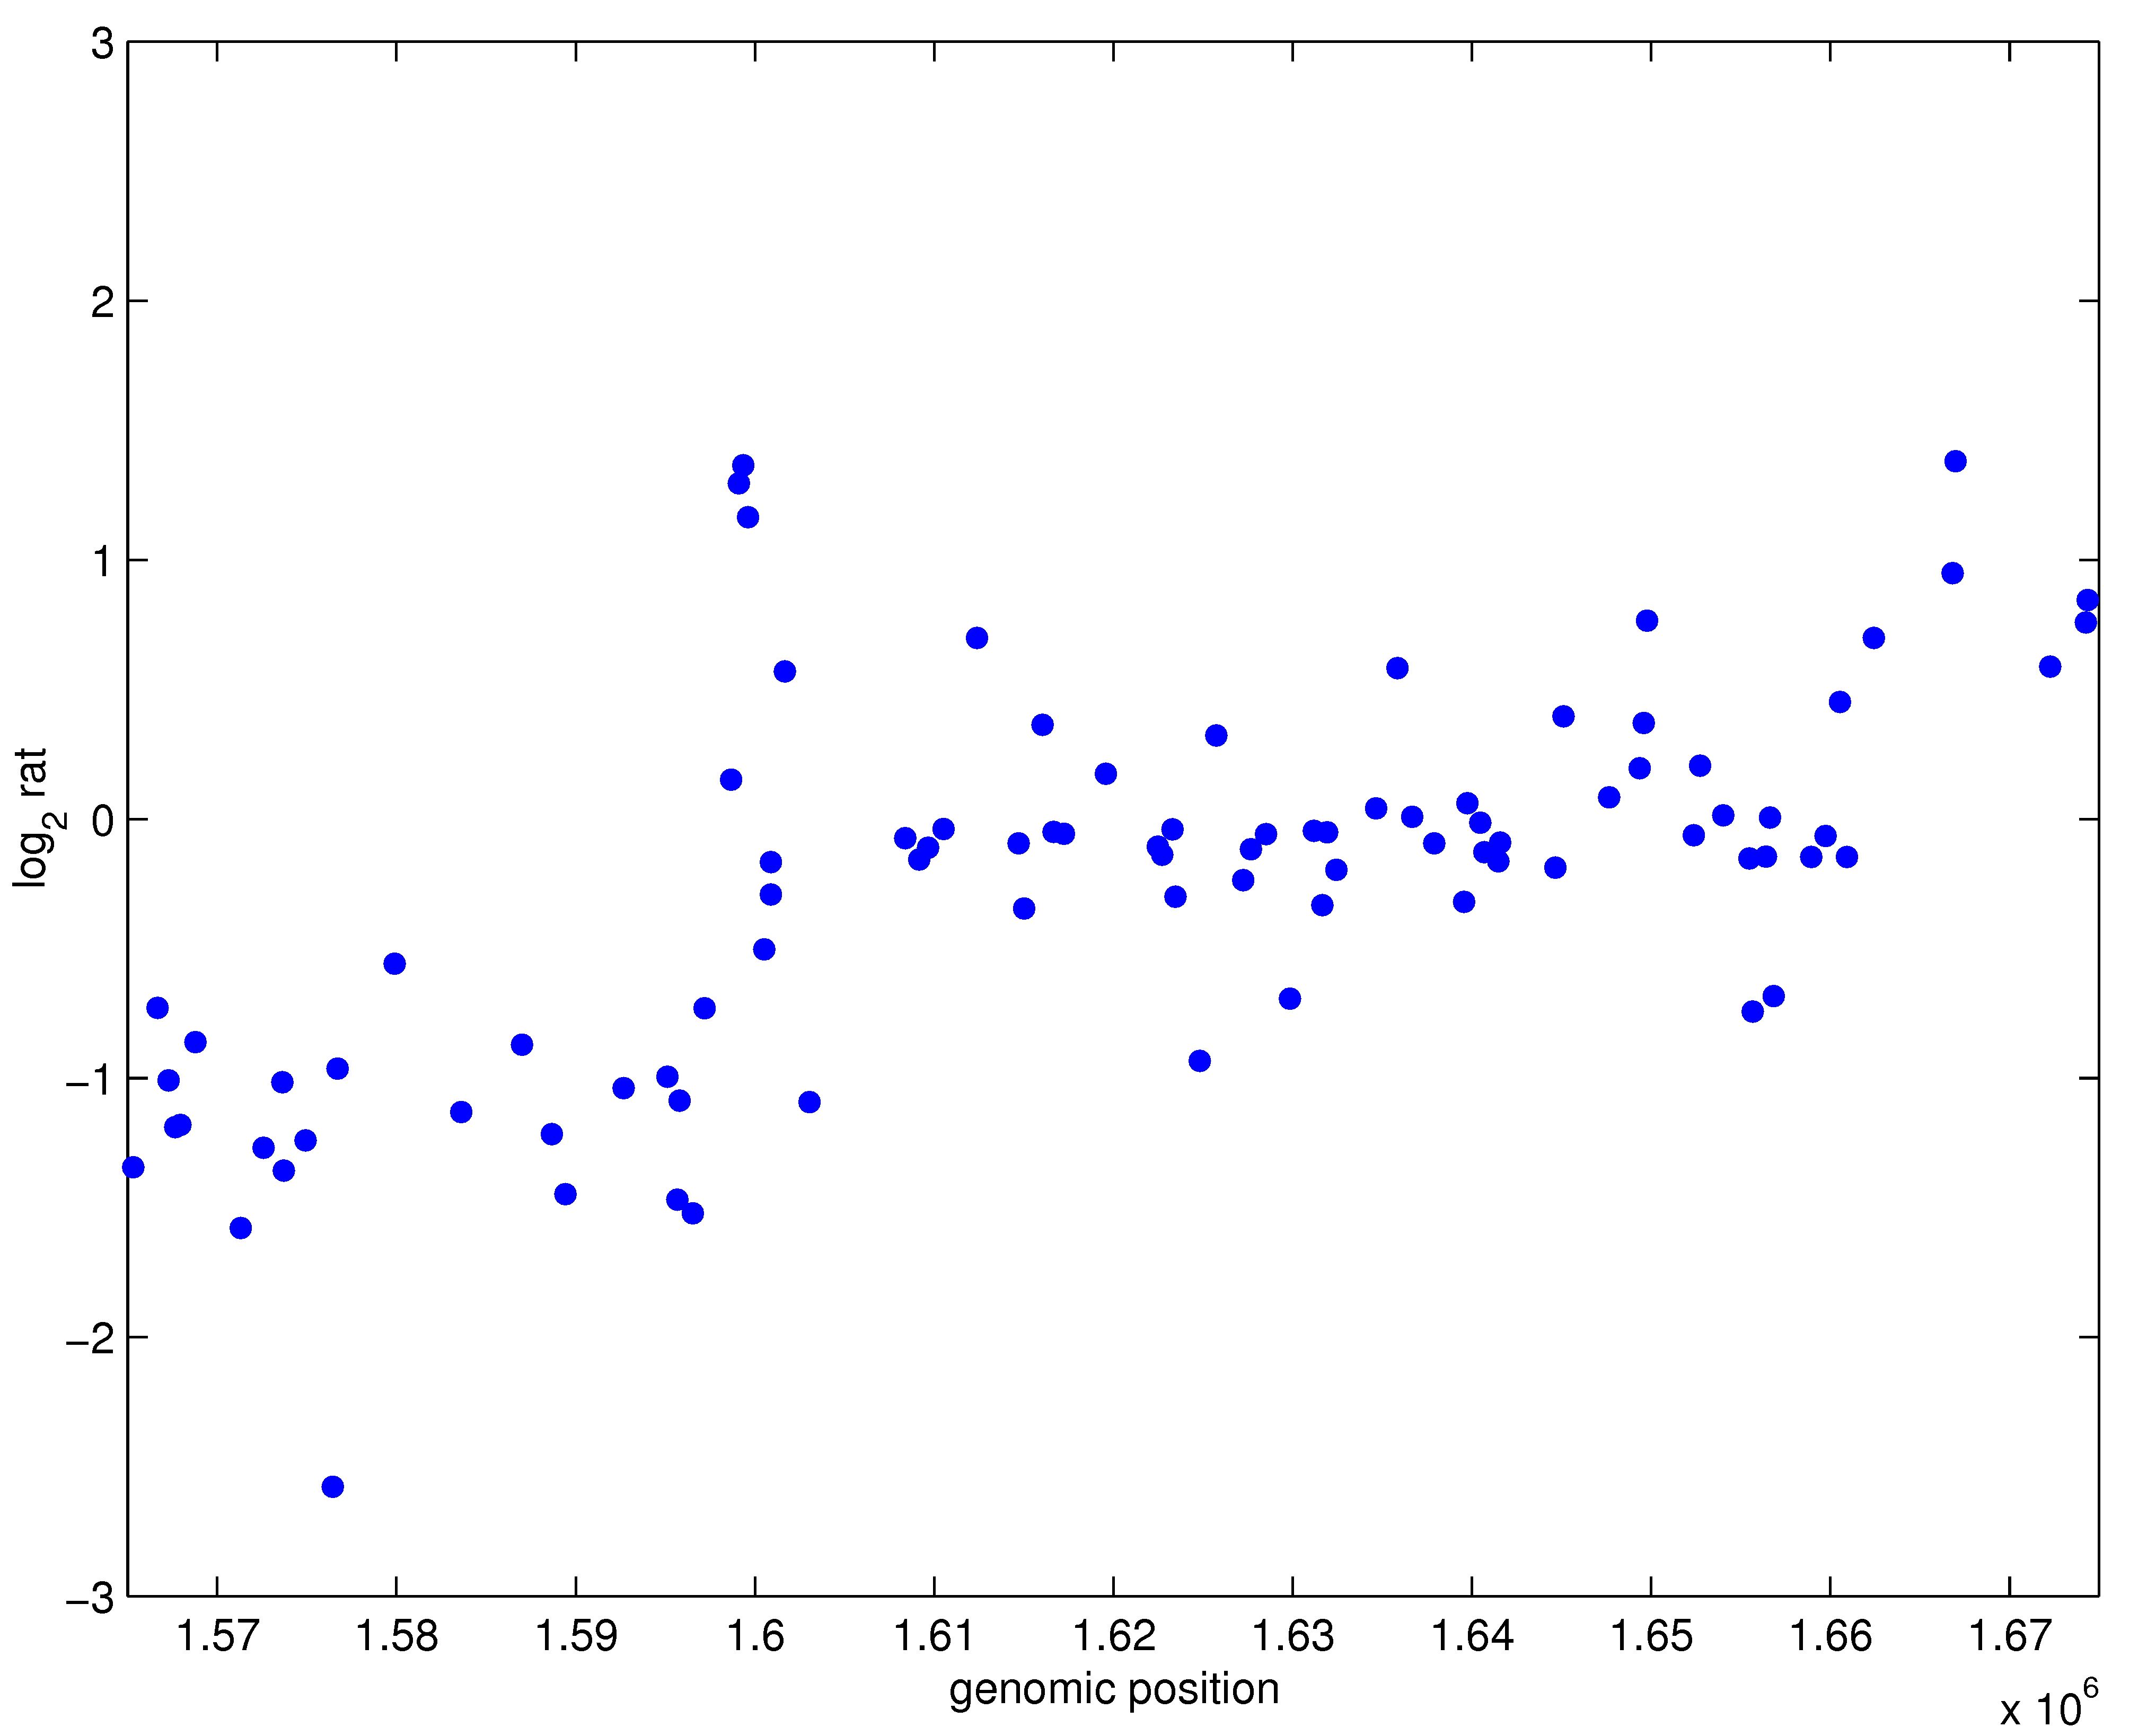
\epsfig{file = ../Figures/raw_profile_example.eps, clip=, width=12cm}
  \end{tabular}
  &
  \begin{tabular}{p{12cm}}
    CGH data analysis aim at recovering the signal to localise the
    breakpoints: \\
    \\
    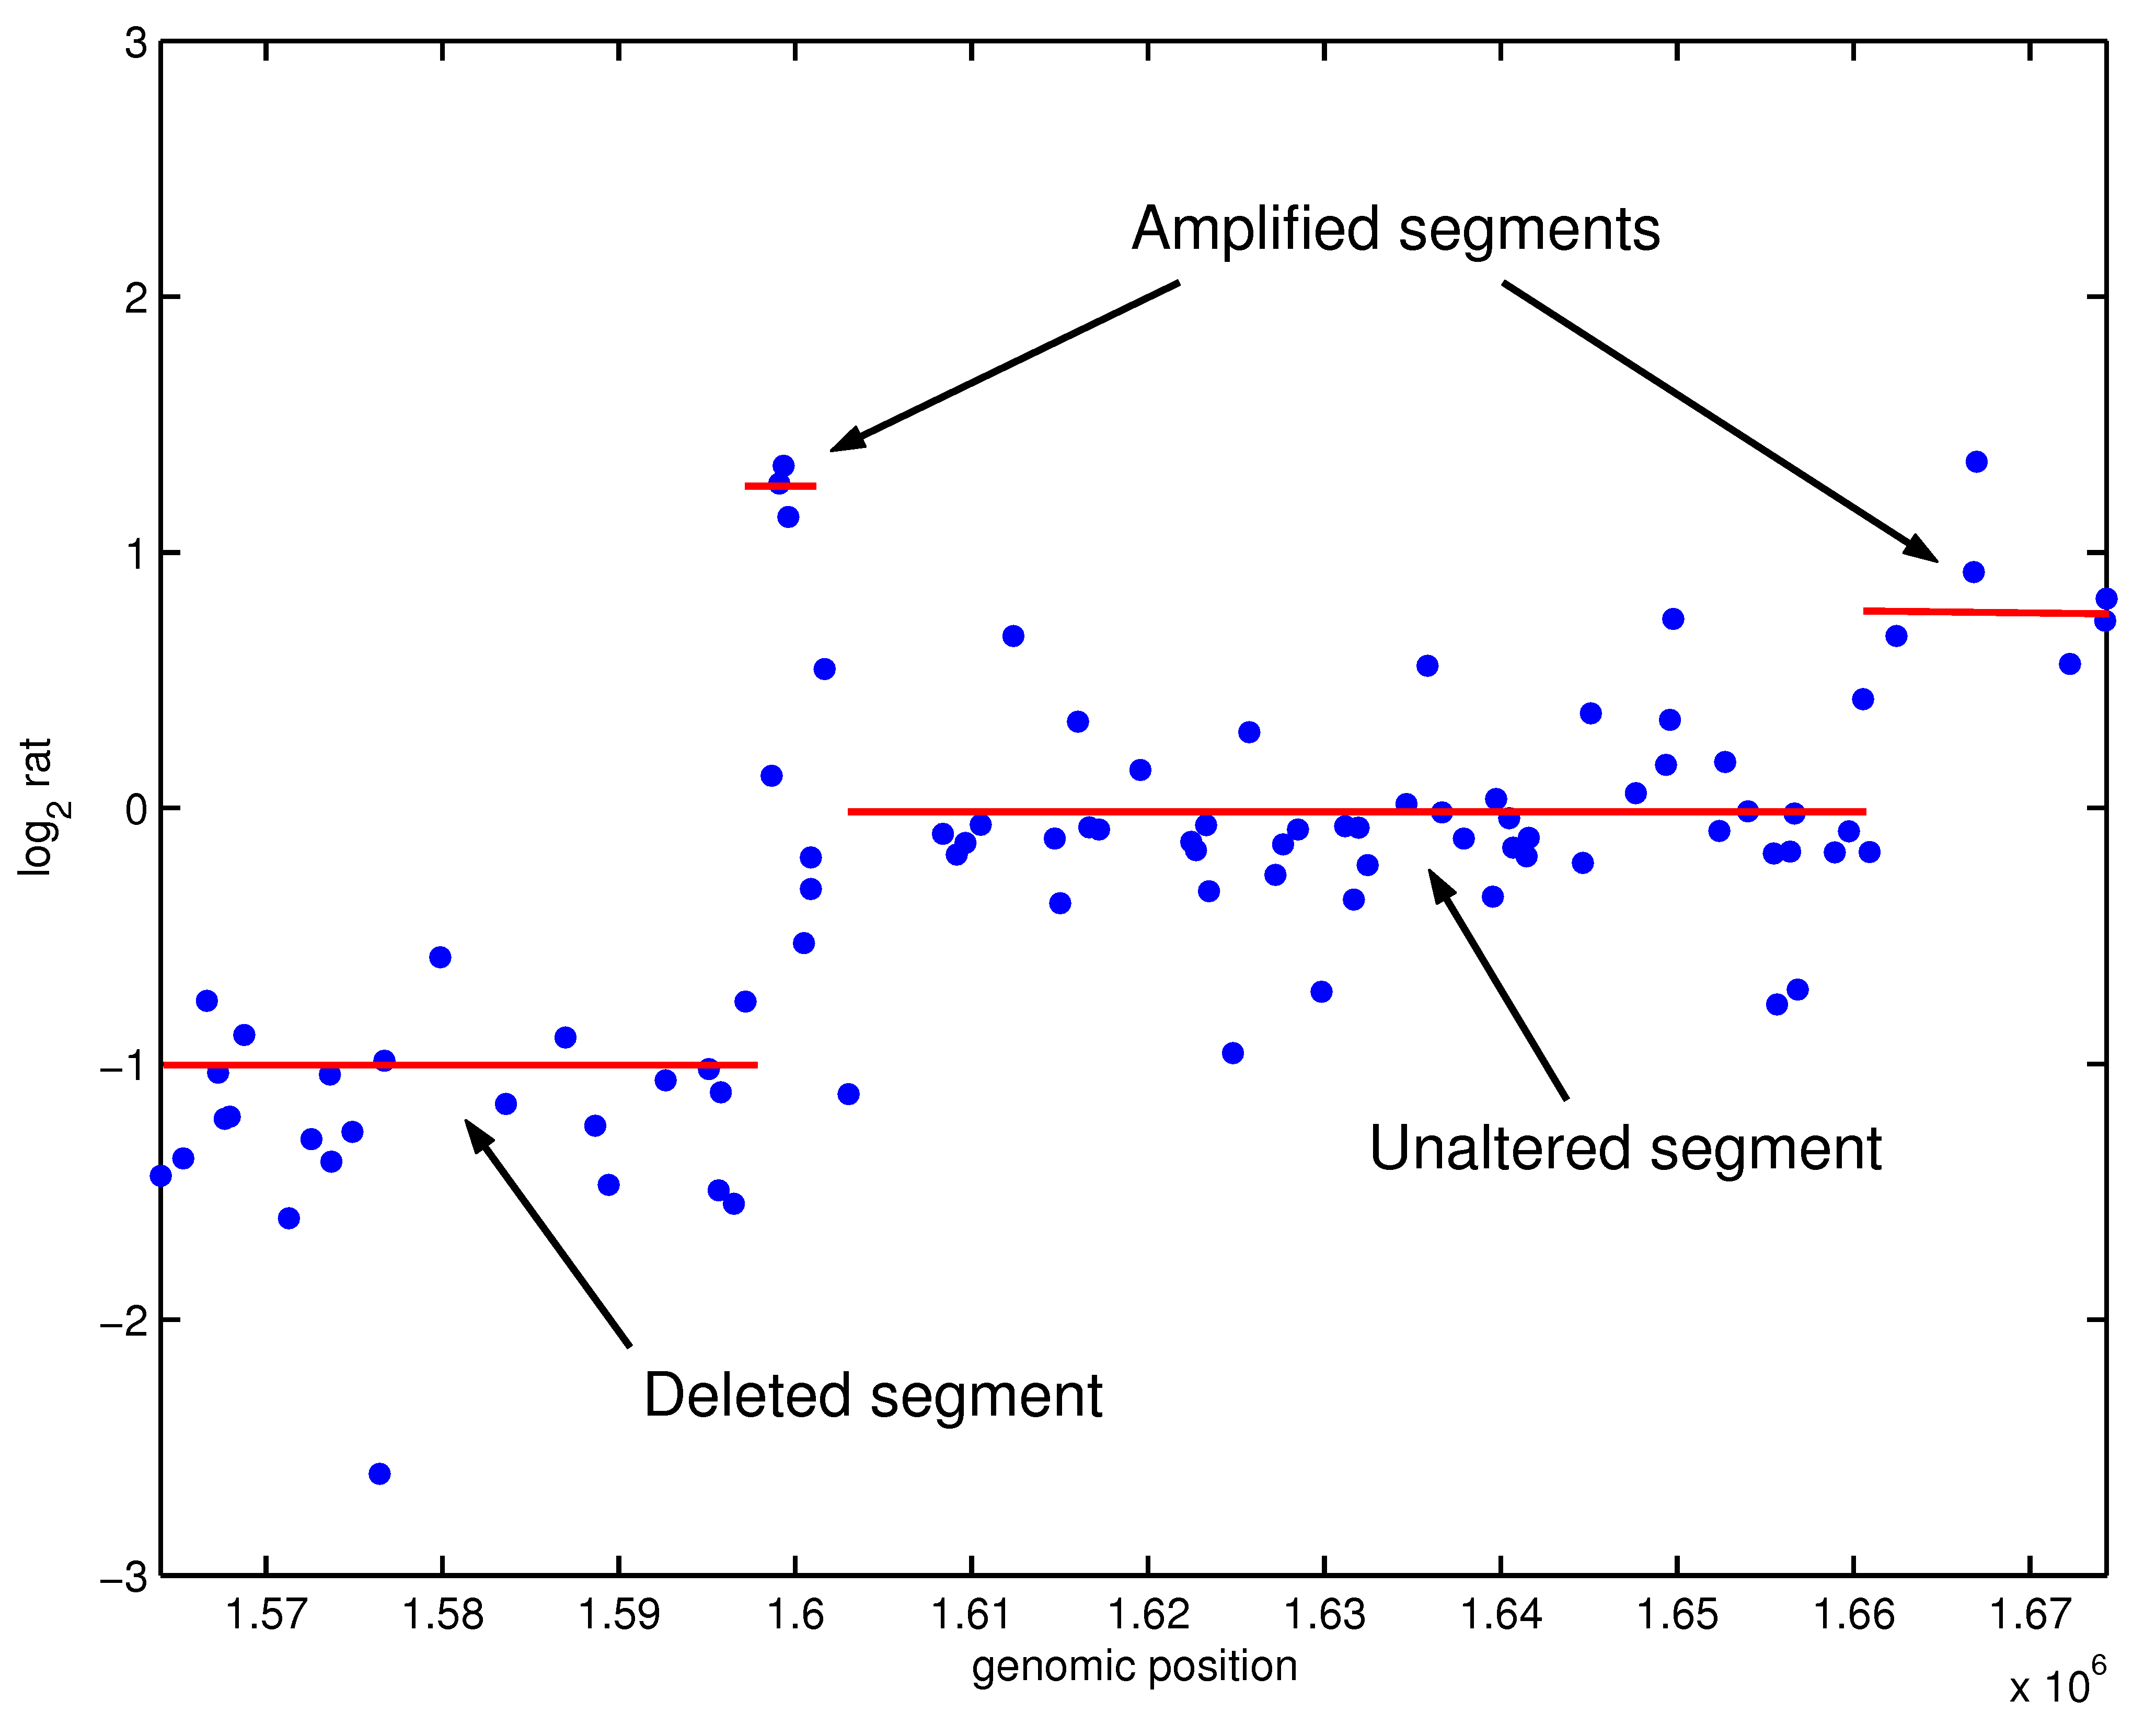
\epsfig{file = ../Figures/profile_example.eps, clip=,
  bbllx=60, bblly=196, bburx=543, bbury=586, width=12cm}
  \end{tabular}
\end{tabular}

\paragraph{Need for} efficient algorithms and model selection techniques.

%%%%%%%%%%%%%%%%%%%%%%%%%%%%%%%%%%%%%%%%%%%%%%%%%%%%%%%%%%%%%%%%%%%%%%
\newpage
\section{Chromatine Immuno-Precipitation}
%%%%%%%%%%%%%%%%%%%%%%%%%%%%%%%%%%%%%%%%%%%%%%%%%%%%%%%%%%%%%%%%%%%%%%

\hspace{-2.25cm}
\begin{tabular}{cc}
  \begin{tabular}{p{12cm}}
    Gene expression is controlled by \emphase{epi-genetic mecanisms}
      \begin{itemize}
    \item \vspace{-0.5cm} Transcription factors and co-factors
    \item \vspace{-0.5cm} DNA methylation
    \item \vspace{-0.5cm} Histone modifications 
  %$\rightarrow$ alter chromatin structure $\rightarrow$ alter gene expression
    \end{itemize} \\
    \\
    \paragraph{ChIP-chip technology:} \\
    \\
    Target = Product of immuno-precipitation \\
    \\
    Probes = Numerous sequences covering the whole genome (tilling array)
  \end{tabular}
  &
  \begin{tabular}{p{12cm}}
    \epsfig{file = ../Figures/Chip-chip.ps, width=14cm,height=14cm, clip=}
  \end{tabular}
\end{tabular}

%%%%%%%%%%%%%%%%%%%%%%%%%%%%%%%%%%%%%%%%%%%%%%%%%%%%%%%%%%%%%%%%%%%%%%
\newpage
\subsection{An unsupervised classification problem}

\noindent We aim discovering which probes are normal and which are
enriched.  \emphase{Mixture models} provide a natural framework to
achieve this goal.

\hspace{-2.25cm}
\begin{tabular}{cc}
  \begin{tabular}{p{12cm}}
    \paragraph{Log-ratio = log(IP / Input).} \\
    \\
    \epsfig{file =
      ../Figures/BelleDistribution.ps, width=10cm, height=5cm, clip=} 
    %\includegraphics[scale=0.5]{../Figures/BelleDistribution.ps}
    \epsfig{file =
      ../Figures/Graph_Histogramme_LogRatio_MoyDye_Rep2_chr4.ps,
    width=5cm, height=10cm, angle=-90, clip=} 
  \end{tabular}
  &
  \begin{tabular}{p{12cm}}
    \paragraph{Scatter plot of log(IP) vs log(Input).} \\
    \\
    \epsfig{file = ../Figures/Nuage.ps,width=10cm,height=10cm,clip=}
    \\ \\
  \end{tabular}
\end{tabular}

\noindent Modelling the joint distribution of (IP, Input) is probably
more efficient.

%%%%%%%%%%%%%%%%%%%%%%%%%%%%%%%%%%%%%%%%%%%%%%%%%%%%%%%%%%%%%%%%%%%%%%
\newpage
\section{Next Sequencing Generation: Solexa Technology}
%%%%%%%%%%%%%%%%%%%%%%%%%%%%%%%%%%%%%%%%%%%%%%%%%%%%%%%%%%%%%%%%%%%%%%

\noindent \emphase{Sequencing techniques} now aim at replacing microarrays.
$$
\begin{tabular}{ccc}
  \epsfig{file = ../Figures/SolexaTechnology-1.ps, bbllx=68, bblly=456,
    bburx=214, bbury=706, clip=, width=8cm, height=10cm}
  &
  \epsfig{file = ../Figures/SolexaTechnology-1.ps, bbllx=381, bblly=150,
    bburx=526, bbury=398, clip=, width=8cm, height=10cm}
  &
  \epsfig{file = ../Figures/SolexaTechnology-2.ps, bbllx=381, bblly=484,
    bburx=527, bbury=733, clip=, width=8cm, height=10cm}
\end{tabular}
$$
\begin{itemize}
\item \vspace{-0.5cm} One experiment provides $10^7$ fragments of
  25-50 bp and 1 Tb of data!!! 
\item \vspace{-0.5cm} Measurement are basically counts (instead of continuous
  values) associated to position along the genome. 
\end{itemize}

%%%%%%%%%%%%%%%%%%%%%%%%%%%%%%%%%%%%%%%%%%%%%%%%%%%%%%%%%%%%%%%%%%%%%%
\newpage
\subsection{Same purpose as microarrays...}

Most questions addressed with
microarrays can be addressed with sequencing:
\begin{itemize}
\item \vspace{-0.5cm} Gene expression
\item \vspace{-0.5cm} Chromosomal aberrations 
\item \vspace{-0.5cm} ChIP (ChIP-chip $\rightarrow$ ChIP-seq)
\item \vspace{-0.5cm} ...
\end{itemize}

%%%%%%%%%%%%%%%%%%%%%%%%%%%%%%%%%%%%%%%%%%%%%%%%%%%%%%%%%%%%%%%%%%%%%%
\subsection{... Plus others} 

\paragraph{Genome re-sequencing.} It should be possible to re-sequence
the genome of a species with known genome sequence to \emphase{correct
  errors} or to \emphase{explore its genomic variability}.

\paragraph{Meta-genome.} Many media gather hundreds of species that
  can not be isolated (human gut, soil, etc.). The meta-genome of such
  a media is the set of the genomes of all present species. Exploring
  the meta-genome should give insight about the \emphase{present species},
  their \emphase{relative abundance}, their \emphase{diversity}, etc.

%%%%%%%%%%%%%%%%%%%%%%%%%%%%%%%%%%%%%%%%%%%%%%%%%%%%%%%%%%%%%%%%%%%%%%
%%%%%%%%%%%%%%%%%%%%%%%%%%%%%%%%%%%%%%%%%%%%%%%%%%%%%%%%%%%%%%%%%%%%%%
\newpage
\chapter{Many Different Kinds of Data} 
%%%%%%%%%%%%%%%%%%%%%%%%%%%%%%%%%%%%%%%%%%%%%%%%%%%%%%%%%%%%%%%%%%%%%%
%%%%%%%%%%%%%%%%%%%%%%%%%%%%%%%%%%%%%%%%%%%%%%%%%%%%%%%%%%%%%%%%%%%%%%

\hspace{-2.25cm}
\begin{tabular}{cc}
  \begin{tabular}{p{12cm}}
    2 hybrid technology gives evidence for in-vitro \emphase{protein-protein
      interactions}. \\
    \emphase{$\rightarrow$} Data are structured as a \emphase{graph}.
  \end{tabular}
  & 
  \begin{tabular}{p{12cm}}
    \epsfig{file=../Figures/2hybridTechnology.ps, bbllx=91, bblly=590,
      bburx=230, bbury=662, width=12cm, height=5cm, clip=} 
  \end{tabular}
  \\
  \begin{tabular}{p{12cm}}
    \epsfig{file=../Figures/DataIntegration.ps, bbllx=255, bblly=447,
      bburx=332, bbury=517, width=12cm, height=5cm, clip=}
  \end{tabular}
  & 
  \begin{tabular}{p{12cm}}
    Phylogeny gives information about \emphase{gene's and protein's
      history}. \\
    \emphase{$\rightarrow$} Data are structured as a \emphase{tree}.  
  \end{tabular}
  \\
  \begin{tabular}{p{12cm}}
    In situ hybridisation tells us in \emphase{which cell compartment}
    genes are actually expressed.\\
    \emphase{$\rightarrow$} Data are \emphase{cellular location} or
    spatial coordinates.      
  \end{tabular}
  & 
  \begin{tabular}{p{12cm}}
    \epsfig{file=../Figures/DataIntegration.ps, bbllx=345, bblly=447,
      bburx=422, bbury=517, width=12cm, height=5cm, clip=}   
  \end{tabular}
\end{tabular}


%%%%%%%%%%%%%%%%%%%%%%%%%%%%%%%%%%%%%%%%%%%%%%%%%%%%%%%%%%%%%%%%%%%%%%
\newpage
\section{Extracting Information from All This: \refer{J.-Ph. Vert}{}}
%%%%%%%%%%%%%%%%%%%%%%%%%%%%%%%%%%%%%%%%%%%%%%%%%%%%%%%%%%%%%%%%%%%%%%

\paragraph{Data integration.} Gathering data with \emphase{different nature and
  structure} is a major challenge of modern biology.

\paragraph{Typical question.} Are we able to fit a model such as
$$
\Pr\left\{
  \begin{tabular}{p{6cm}}
    protein $A$ interacts with protein $B$
  \end{tabular}
\right\}
=
f \left( 
  \begin{tabular}{p{12cm}}
    gene expression + phylogeny + in-situ hybridisation + mass
    spectrometry 
  \end{tabular}
\right)
$$

\paragraph{Kernel methods} provide an efficient framework to achieve
this task.
\begin{itemize}
\item \vspace{-0.5cm} Kernels can be viewed as \emphase{scalar
    product} in very general feature spaces.
\item \vspace{-0.5cm} They provide \emphase{similarity measures} for
  data with (almost) any structure.
\item \vspace{-0.5cm} Many \emphase{classical analyses} can then be
  adapted: kernel-PCA, kernel-LDA.
\item \vspace{-0.5cm} Other efficient strategies are defined in this
  framework: SVM.
\end{itemize}


%%%%%%%%%%%%%%%%%%%%%%%%%%%%%%%%%%%%%%%%%%%%%%%%%%%%%%%%%%%%%%%%%%%%%%
%%%%%%%%%%%%%%%%%%%%%%%%%%%%%%%%%%%%%%%%%%%%%%%%%%%%%%%%%%%%%%%%%%%%%%
\newpage
\chapter{Networks} 
\bigskip
%%%%%%%%%%%%%%%%%%%%%%%%%%%%%%%%%%%%%%%%%%%%%%%%%%%%%%%%%%%%%%%%%%%%%%
%%%%%%%%%%%%%%%%%%%%%%%%%%%%%%%%%%%%%%%%%%%%%%%%%%%%%%%%%%%%%%%%%%%%%%

%%%%%%%%%%%%%%%%%%%%%%%%%%%%%%%%%%%%%%%%%%%%%%%%%%%%%%%%%%%%%%%%%%%%%%
\section{Systems Biology}
%%%%%%%%%%%%%%%%%%%%%%%%%%%%%%%%%%%%%%%%%%%%%%%%%%%%%%%%%%%%%%%%%%%%%%

\noindent The final goal is to understand the \emphase{interactions
  between all the component} present in a cell. Systems biology aims
at studying the cell as a whole, i.e. as a system involving many
elements.  

These interactions are often seen as networks:
\begin{itemize}
\item \vspace{-0.5cm} \emphase{Regulation network:} Which gene regulates which?
\item \vspace{-0.5cm} \emphase{Interaction network:} Which protein interacts
  with which?
\item \vspace{-0.5cm} \emphase{Metabolic pathway:} Which reaction is downstream
  from another? \\
  Which enzyme catalyses each of them?
\item \vspace{-0.5cm} \emphase{Dynamic network:} Given the
  stoichiometry and all chemical constants, how the system is going to
  evolve?
\end{itemize}

% \hspace{-2.25cm}
% \begin{tabular}{cc}
%   \begin{tabular}{p{12cm}}
%   \end{tabular}
%   &
%   \begin{tabular}{p{12cm}}
%     \epsfig{file = ../Figures/MAPK.ps, clip, width=12cm}
%   \end{tabular}
% \end{tabular}

%%%%%%%%%%%%%%%%%%%%%%%%%%%%%%%%%%%%%%%%%%%%%%%%%%%%%%%%%%%%%%%%%%%%%%
\newpage
\subsection{A metabolic pathway}

\noindent\epsfig{file=../Figures/Mapk.ps, width=25cm, height=16.5cm,
  clip=} 

%%%%%%%%%%%%%%%%%%%%%%%%%%%%%%%%%%%%%%%%%%%%%%%%%%%%%%%%%%%%%%%%%%%%%%
\newpage
\section{Network Inference: \refer{S. Huet}{}}
%%%%%%%%%%%%%%%%%%%%%%%%%%%%%%%%%%%%%%%%%%%%%%%%%%%%%%%%%%%%%%%%%%%%%%

\noindent A first task is to infer these relations from the data we
have.

\paragraph{Typical question:} Can we recover gene regulation from gene   
expression data? 

\paragraph{Gaussian graphical model.} 
\begin{itemize}
\item \vspace{-0.5cm} Denote $X_{gt}$ the expression level of gene $g$
  in replicate $t$ and $\Xbf_t = (X_{1t}, \dots, X_{Gt})$. 
\item \vspace{-0.5cm} Assume that the vectors $\Xbf_t$ are
  i.i.d. $\sim \Ncal(\mubf, \Sigmabf)$, where $\Sigmabf$ is $G \times G$..
\item \vspace{-0.5cm} The non-zeros terms of $\Sigmabf^{-1}$ reveal
  direct correlations (regulations ?) between genes.
\end{itemize}

\paragraph{(Some) statistical issues.} 
\begin{itemize}
\item \vspace{-0.5cm} \emphase{Large $p$, small $n$ situation:} the
  number of genes $G$ is much larger than the number of replicates. \\
  $\Rightarrow \widehat{\Sigmabf}$ is necessarily singular.
\item \vspace{-0.5cm} \emphase{Multiple testing / Model selection:}
  The network is assumed to be sparse. \\
  We want to know which $\sigma^{-1}_{gh}$ are non-zero, avoiding
  false positives.
\end{itemize}

%%%%%%%%%%%%%%%%%%%%%%%%%%%%%%%%%%%%%%%%%%%%%%%%%%%%%%%%%%%%%%%%%%%%%%
\newpage
\section{Network analysis: \refer{J.-J. Daudin}{}}
%%%%%%%%%%%%%%%%%%%%%%%%%%%%%%%%%%%%%%%%%%%%%%%%%%%%%%%%%%%%%%%%%%%%%%

\hspace{-2.25cm}
\begin{tabular}{cc}
  \begin{tabular}{p{12cm}}
    Even when the network is observed, analysing its structure
    is still an issue. \\
    \\
    One may look for some \\
    \\
    \emphase{Global structure} (groups of nodes with similar connectivity
    profile) \\
    \\
    \emphase{Local structure} (motifs or patterns that are recurrent
    throughout the network). 
  \end{tabular}
  &
  \begin{tabular}{p{12cm}}
        \epsfig{file = ../Figures/Barabasi6.ps, clip=, bbllx=39, bblly=466,
      bburx=351, bbury=754, width=12cm} \\
  \end{tabular}
\end{tabular}

%%%%%%%%%%%%%%%%%%%%%%%%%%%%%%%%%%%%%%%%%%%%%%%%%%%%%%%%%%%%%%%%%%%%%%
\newpage

\hspace{-2.25cm}
\begin{tabular}{cc}
  \begin{tabular}{p{12cm}}
    \subsection{Global structure} \\
    \\
    Mixture models allow to perform unsupervised clustering of the
    nodes. \\
    \\
    Unstructured $\rightarrow$ Structured 
    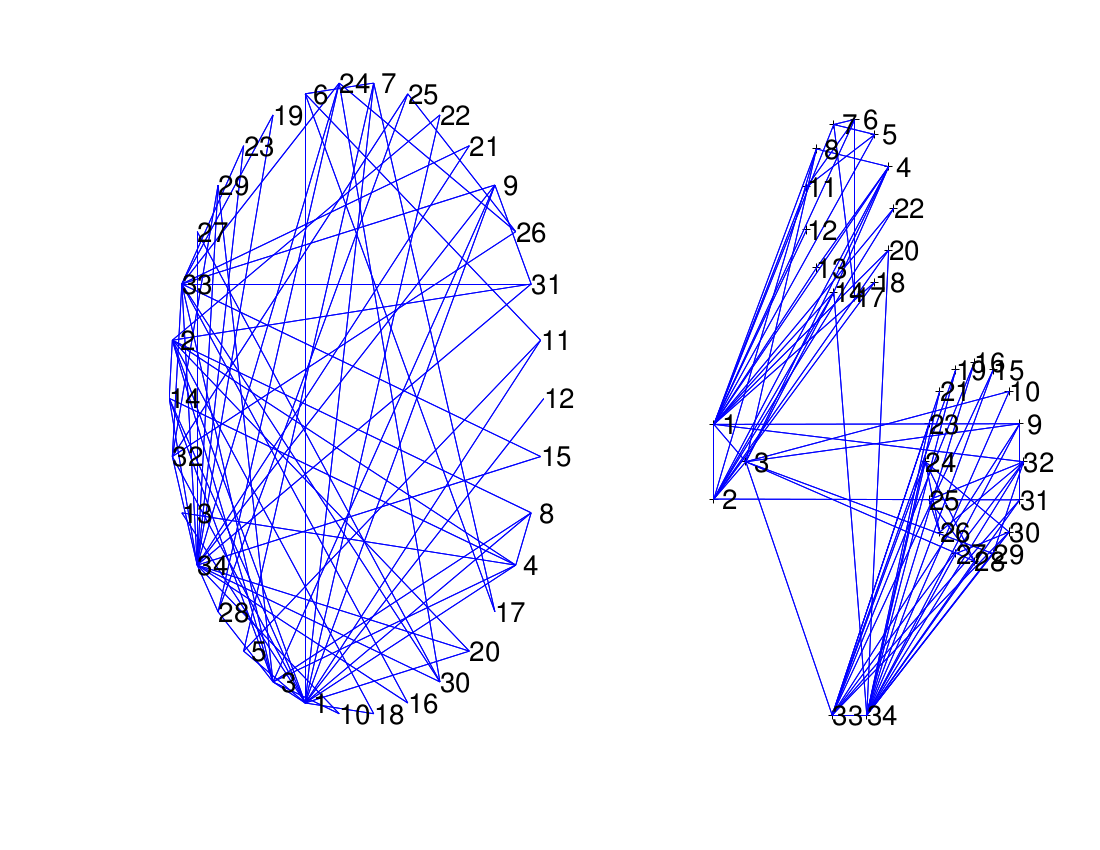
\epsfig{file = ../Figures/Karate-Graph.eps, clip=, width=4cm,
      height=5.8cm, angle=270, bbllx=48, bblly=120, bburx=526,
      bbury=420} 
    \quad
    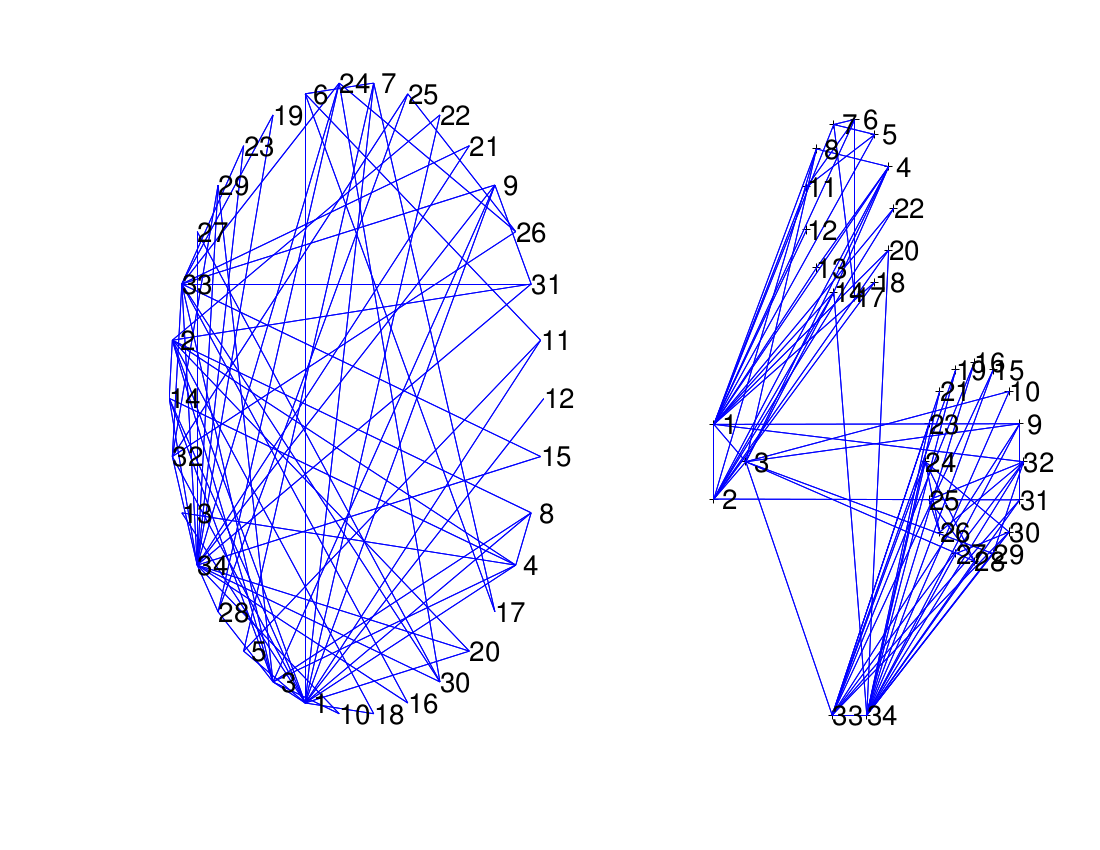
\epsfig{file = ../Figures/Karate-Graph.eps, clip=, width=4cm,
      height=5cm, angle=270, bbllx=48, bblly=510, bburx=526,
      bbury=760} \\
    \\ \\
    \paragraph{Statistical issue.} \\
    Due to very intricate dependencies, the popular E-M algorithm can
    not be used. \\ 
    \\
    $\rightarrow$ \emphase{Variational} approximation
  \end{tabular}
  &
  \begin{tabular}{p{12cm}}
    \subsection{Local structure} \\
    \\
    Over-represented motif reveal the local behaviour of the
    network. \\
    \\
    \epsfig{file=../FIGURES/RegulationMotifs.ps, bbllx=83, bblly=506,
      bburx=288, bbury=600, clip=, width=5.5cm}  
    \epsfig{file=../FIGURES/RegulationMotifs.ps, bbllx=83, bblly=338,
      bburx=288, bbury=431, clip=, width=5.5cm}  \\
    \\ \\
    \paragraph{Statistical issues.}
    \begin{itemize}
    \item \vspace{-0.5cm} Precisely define a motif and its
      occurrences. 
    \item \vspace{-0.5cm} Derive the distribution of the number of
      occurrences.
    \item \vspace{-0.5cm} Find a relevant random graph model as
      reference model.
    \end{itemize}
  \end{tabular}
\end{tabular}


%%%%%%%%%%%%%%%%%%%%%%%%%%%%%%%%%%%%%%%%%%%%%%%%%%%%%%%%%%%%%%%%%%%%%%
\newpage
\section{Statistical Methods for Post-Genomic Data}
%%%%%%%%%%%%%%%%%%%%%%%%%%%%%%%%%%%%%%%%%%%%%%%%%%%%%%%%%%%%%%%%%%%%%%

\vspace{2cm}
\subsection{7th Workshop:}
 
\begin{itemize}
\item in Paris (AgroParisTech), 
\item the 29-30 January 2009
\end{itemize}

$$
\text{\emphase{\url{http://www.lsp.ups-tlse.fr/Biopuces/SMPGD09/ }}}
$$

%%%%%%%%%%%%%%%%%%%%%%%%%%%%%%%%%%%%%%%%%%%%%%%%%%%%%%%%%%%%%%%%%%%%%%
%%%%%%%%%%%%%%%%%%%%%%%%%%%%%%%%%%%%%%%%%%%%%%%%%%%%%%%%%%%%%%%%%%%%%%
%%%%%%%%%%%%%%%%%%%%%%%%%%%%%%%%%%%%%%%%%%%%%%%%%%%%%%%%%%%%%%%%%%%%%%
%%%%%%%%%%%%%%%%%%%%%%%%%%%%%%%%%%%%%%%%%%%%%%%%%%%%%%%%%%%%%%%%%%%%%%
\end{document}
%%%%%%%%%%%%%%%%%%%%%%%%%%%%%%%%%%%%%%%%%%%%%%%%%%%%%%%%%%%%%%%%%%%%%%
%%%%%%%%%%%%%%%%%%%%%%%%%%%%%%%%%%%%%%%%%%%%%%%%%%%%%%%%%%%%%%%%%%%%%%
%%%%%%%%%%%%%%%%%%%%%%%%%%%%%%%%%%%%%%%%%%%%%%%%%%%%%%%%%%%%%%%%%%%%%%
%%%%%%%%%%%%%%%%%%%%%%%%%%%%%%%%%%%%%%%%%%%%%%%%%%%%%%%%%%%%%%%%%%%%%%

\hspace{-2.25cm}
\begin{tabular}{cc}
  \begin{tabular}{p{12cm}}
  \end{tabular}
  &
  \begin{tabular}{p{12cm}}
  \end{tabular}
\end{tabular}
